\chapter{Series-Generation in DNA}
This chapter will deal with the general series-generation mechanisms in DNA and how to use them. Different approaches and configurations will be shown on examples to give a quick and easy insight into DNA usage.

\section{General}
A series in DNA is composed of several objects:

\begin{center}
\begin{math}
S = (GraphGenerator, BatchGenerator, Metric[], SeriesDir, SeriesName)
\end{math}
\end{center}

The generation process uses a GraphGenerator to generate the graph and a BatchGenerator to
compile graph changes into batches. Figure \ref{fig:dna-architecture} illustrates the architecture and components of DNA. It offers a variety of different Graph- and BatchGenerators for different graphs and purposes. Due to the nature of dynamic graphs, metrics can either calculate their values based on initial information and additional updates or do a full recompute after each update. During generation DNA will store statistics, runtimes and computed data in series objects. A series contains one or more runs, each of which represent one separate simulation. A run is divided into several batches, which contain statistics, runtimes and metric datas, see \ref{fig:fs-struct-gen}. The \textit{aggr}-directory envelopes aggregated data of all runs contained in the specific series. For more details on the DNA architecture and theoretical background check the DNA paper \cite{dna-paper13}.

\begin{figure} [h]
\centering
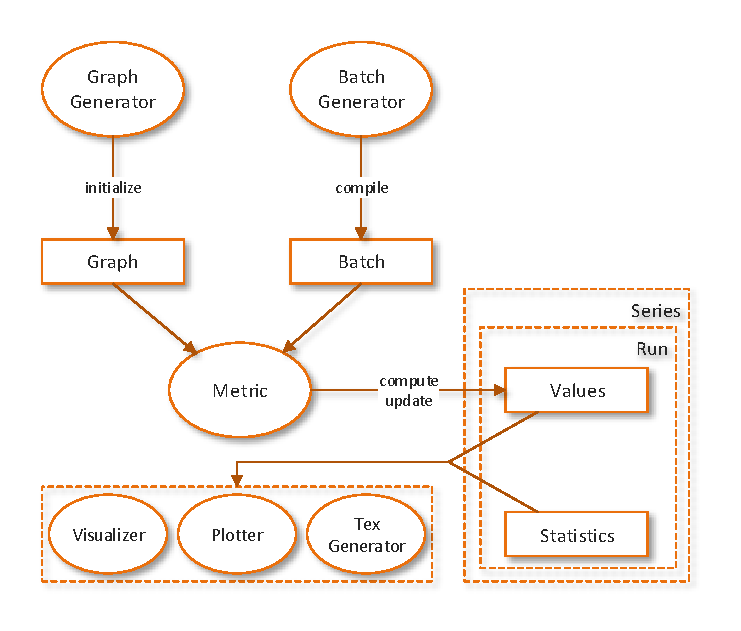
\includegraphics [scale=1.2] {images/dna-architecture}
\caption{DNA architecture and components.}
\label{fig:dna-architecture}
\end{figure}

\begin{figure} [h]
\centering
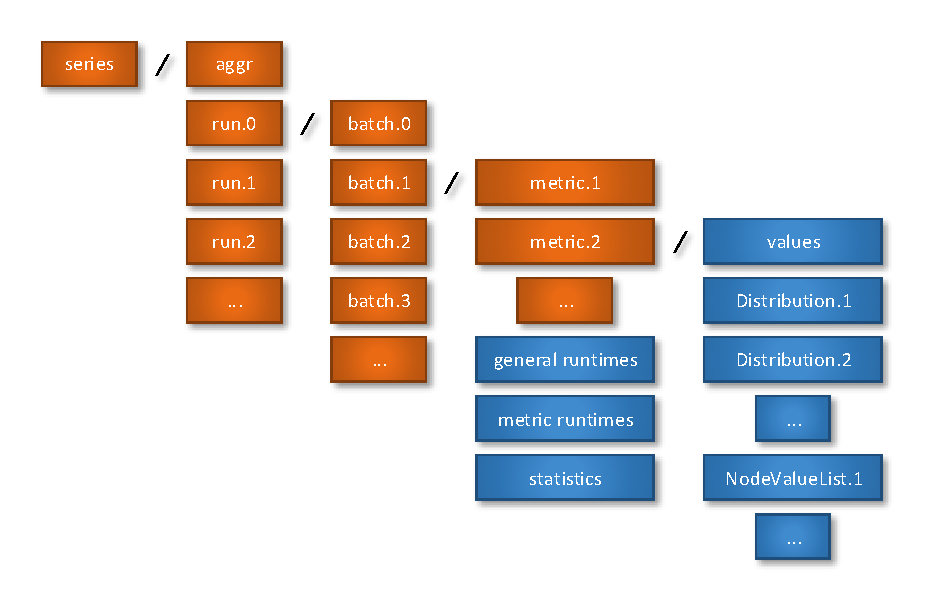
\includegraphics [scale=1] {images/fs-struct-gen}
\caption{General filesystem structure for storing the results of a series.}
\label{fig:fs-struct-gen}
\end{figure}


\section{Getting started}
The usual workflow is pretty simple. First one initializes a GraphGenerator, BatchGenerator and an array of metrics. Then a Series object is initialized with these inputs. The second step is the generation itself: Each Series-object has several generation-methods for different purposes. 

\subsection{First approach}
The example in \ref{code:example1} shows how one could generate a random, undirected graph with initially 100 nodes and 300 edges. With each batch 5 nodes and 20 edges are being randomly added while also 15 edges are being removed. The metrics \textit{DegreeDistributionR} (recomputed) and \textit{UndirectedClusteringCoefficientU} (updated) are chosen to be computed. The resulting filesystem structure can be seen in figure \ref{fig:fs-struct-val}.
\begin{figure} [h]
\begin{lstlisting}
public static void main(String[] args) throws AggregationException,
		IOException, MetricNotApplicableException,
		InterruptedException {
	String seriesDir = "data/series/";

	// initialization, 100 nodes and 300 edges
	GraphGenerator gg1 = new RandomGraph(GDS.undirected, 100, 300);
	
	// 5 nodes-added, 0 nodes-removed, 20 edges-added, 15 edges-removed
	BatchGenerator bg1 = new RandomBatch(5, 0, 20, 15);
	
	// choose metrics
	Metric[] m1 = new Metric[] { new DegreeDistributionR(),
			new UndirectedClusteringCoefficientU() };

	// create series and generate it
	Series s = new Series(gg1, bg1, m1, seriesDir, "series");
	
	// generate 2 runs with 100 batches each
	SeriesData sd = s.generate(2, 100);
}
\end{lstlisting}
\caption{Simple generation example.}
\label{code:example1}
\end{figure}
\begin{figure} [h]
\centering
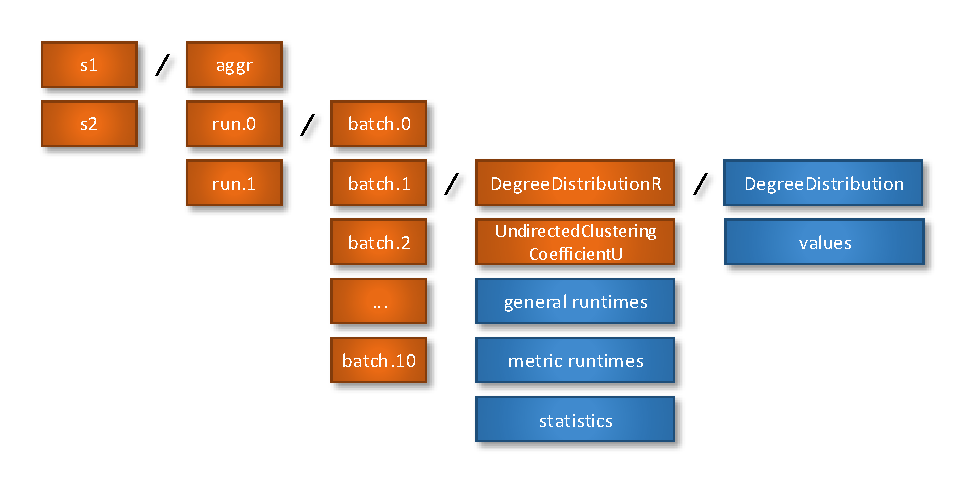
\includegraphics [scale=1] {images/fs-struct-val}
\caption{Filesystem structure for example \ref{code:example1}.}
\label{fig:fs-struct-val}
\end{figure}

\section{Auto-generated extra-values}
The DNA is able to compute additional extra values for distributions and nodevaluelists. This is enabled by default and can be finely configured in the \textit{settings.properties} configuration file. These include \textit{minimum}, \textit{maximum}, \textit{median}, \textit{average}, \textit{binsize}, \textit{denominator} and additional upper bounds for distributions. Please note, that the median will return the value, which divides the data in two even 50\% portions. If such a value does not exist, e.g. when the number of data points is even, the returned value will be the mean between the two median points. 

Consider the following example:\\
The metric \textit{DegreeDistributionR} calculates a distribution \textit{DegreeDistribution}. In each batch DNA will automatically compute the additional values \textit{DegreeDistribution\textunderscore AVG}, \textit{DegreeDistribution\textunderscore MAX}, \textit{DegreeDistribution\textunderscore MED} and \textit{DegreeDistribution\textunderscore MIN} based on the distribution. Note: It is also possible to generate \textit{DegreeDistribution\textunderscore DENOMINATOR}, \textit{DegreeDistribution\textunderscore BINSIZE} and additional upper bounds. However, this is disabled by default and may be enabled on demand.

\subsection{Upper bounds}
The minimum and maximum of a distribution may not be very meaningful in a lot of cases.  Therefore, additional upper bounds can be generated by DNA. For instance, one may be interested in how the majority of values is distributed. This can be achieved by computing the upper bound for $X$\% of the data. The upper bound of 95\% will compute a value, which is a upper bound for 95\% of the data. The generation of upper bounds is disabled by default but can be enabled by setting:
\begin{lstlisting}
Config.overwrite("GENERATE_DISTRIBUTION_PERCENT_VALUES", "true")
\end{lstlisting}
Furthermore, one can explicitly specify, which bounds will be computed by setting a list of integers (in String format delimited by ','). For instance, computing the upper bound for 95\% and 60\% will look like this:
\begin{lstlisting}
Config.overwrite("EXTRA_VALUE_DISTRIBUTION_PERCENT", "95, 60")
\end{lstlisting}



 